% !TeX encoding = UTF-8
\documentclass[12pt]{article}

%%% 
\usepackage{hyperref}

\usepackage{amsmath} 
\usepackage{amssymb}
\usepackage{amsfonts}
\usepackage{amsthm}
\usepackage{graphicx}
\usepackage{xcolor}

\textwidth 175mm \textheight 230mm \topmargin -10mm \oddsidemargin
-5mm


%%% Теоремы и утверждения
\newtheorem{proposition}{Proposition}
\newtheorem{lemma}{Lemma}
\newtheorem{theorem}{Theorem}
\newtheorem{definition}{Definition}
\newtheorem{corollary}{Corollary}

\theoremstyle{definition}
\newtheorem*{demo}{Proof}
\newtheorem{remark}{Remark}

%%% Свои операторы
\newcommand\Tr{\operatorname{Tr}}
\newcommand\tr{\operatorname{tr}}
\newcommand\diag{\operatorname{diag}}

\renewcommand\Re{\operatorname{Re}}
\renewcommand\Im{\operatorname{Im}}


\newcommand\bra{\left<}
\newcommand\ket{\right>}
\newcommand{\braket}[1]{\bra#1\ket}
\newcommand{\mf}[1]{\mathfrak{#1}}

\def\al {\alpha}
\def\be {\beta}
\def\br {{\Bbb R}}
\def\bc {{\Bbb C}}
\def\const{\hbox{\rm const}}

\def\de {\delta}
\def\DE {\Delta}
\def\e {\eta}
\def\f {\frac}
\def\ga {\gamma}
\def\GA {\Gamma}
\def\intl {\int\limits}
\def\la {\lambda}
\def\LA {\Lambda}
\def\liml {\lim\limits}
\def\om {\omega}
\def\OM {\Omega}
\def\OB {\ov B}
\def\pr {\partial}
\def\sg {\sigma}
\def\tl {\tilde}
\def\ve {\varepsilon}
\def\vp {\varphi}
\def\th {\theta}
\def\Bbb{\mathbb}

\begin{document}
	\begin{center}
		\Large
		\textbf{Gaussian approximation and its corrections for driven dissipative Kerr model}
		
		\large 
		\textbf{K.Sh. Meretukov}\footnote{Faculty of Physics, Lomonosov Moscow State University, Leninskie Gory, Moscow 119991, Russia\\
			E-mail:\href{mailto:meretukov.khazret@gmail.com}{meretukov.khazret@gmail.com}}
		\textbf{A.E. Teretenkov}\footnote{Department of Mathematical Methods for Quantum Technologies, Steklov Mathematical Institute of Russian Academy of Sciences, ul. Gubkina 8, Moscow 119991, Russia\\ E-mail:\href{mailto:taemsu@mail.ru}{taemsu@mail.ru}}
		\\[1mm]
	\end{center}
	
	\footnotesize
	We develop a general technique to obtain Gaussian approximation and perturbative corrections for bosonic nonlinear models. We apply our technique to the Kerr model in the external classical field with dissipation. Without the external field, it can be solved in the space of density matrices supported at the lowest Fock states. We show that although these solutions are highly non-Gaussian, the moments of the creation and annihilation operators are still described by our approach with high accuracy. In the general case with an external field, we discuss the contribution of our technique to the Gaussian approximation without corrections.
	\normalsize
	
	\section{\label{sec:introduction}Introduction}
	
	The study of systems with Kerr nonlinearity is an actively discussed problem \cite{KerrIntr}. The one-mode dissipative Kerr model has several experimental realizations in semiconductor microcavities, quantum circuits and within optomechanical setups \cite{asjad2023joint}. 
 
 However, when considering the Kerr model, there is a problem with the solution when the number of particles is large \cite{MaslovN}. One of the solution methods is the solution by means of classical stochasticity, but in this case all quantum effects are lost \cite{MaslovSolve}. However, there are techniques to recover some of them  \cite{corney2015non}. Another way to deal with the large number of particles is to assume approximate Gaussian dynamics. This allows at least Gaussian quantum effects to be taken into account. And it is a natural assumption if the initial states are assumed to be Gaussian \cite{joneckis1993quantum, banerjee1993interaction, genoni2009enhancement, roman2015parametric,  bolandhemmat2023quantum}. So we focus our study on approximately Gaussian dynamics.
 
 Also, recently there has been increasing interest in approximations by Gaussian ansatz in other fields, such as quantum spin chain theory, the method we develop may be useful in these fields as well \cite{GaussState}. Also, this approach allows considering not only those cases when at zero order the dynamics is described by a Gaussian channel, but also to consider non-Gaussian channels in real physical systems as nonlinear, but Gaussian channels. This peculiarity is useful in quantum theory of information, since many properties of Gaussian channels are known \cite{Kholevo}.
	
	In Section \ref{sec:GeneralApproch} we develop a general technique for  Gaussian approximation of the dynamics of bosonic modes. We use projection methods with the Kawasaki–Gunton projector \cite{kawasaki1973theory, rau1996reversible, semin2020dynamical}. Recently, it has been formulated for general ansatzes \cite{meretukov2024time}, so it is very natural to apply it to the special case of the Gaussian ansatz. We emphasize that such  a technique allows one not only to describe dynamics under Gaussian approximation, but also to obtain  perturbative corrections to it. We show that correction can be computed in closed form for the Gaussian ansatz.
 
 In Section \ref{sec:ConsideredSystem} we apply our results to the driven dissipative Kerr model \cite{asjad2023joint} in the leading order of perturbation theory. In this case it essentially reduces to the application of the Wick's theorem for the right-hand side of the averaged Heisenberg equations. In Section \ref{sec:feq0} we compare the results of our approach with exact solution in the space of density matrices supported at the lowest Fock states. Even in such a non-Gaussian case we show, that the results predicted by our approach are very close to the exact ones. In Section \ref{sec:Efc} we discuss the corrections to the first-order Gaussian approximation in the case of a weak external field.
	
	
	\section{\label{sec:GeneralApproch}General projection approach for Gaussian approximation and systematic corrections to it}
	
	In this work, we follow the projection approach with the generalized Kawasaki–Gunton projector  \cite{meretukov2024time} for the general ansatz parameterized by averages of some relevant observables. Here, we specify our results for the case, where the ansatz is Gaussian and the relevant observables are creation and annihilation operators and their products.  But,  instead of using parametrization by their averages, we reparameterize  the Gaussian states in a more convenient way in terms of the covariance matrix along with the vector of means.
	
	To formulate our approach explicitly,  let us introduce some compact notation similar to \cite{Dis}. Let  $\mf{a} = (a_1, a_2, \ldots, a_N, a_1^+, a_2^+,\ldots,a_N^+)^T$, where $a_j^{\dagger}$ and $a_j$ are bosonic creation and annihilation operators. The arbitrary sums of quadratic and linear forms in such operators can be written as $\dfrac{1}{2}\mf{a}^TK\mf{a} + g^T\mf{a}$, where $K \in \mathbb{C}^{2N \times 2N}, g \in \mathbb{C}^{2N}$. The canonical commutation relations are written in the form 
	\begin{equation}
		\label{eq:ComRel}
		[f^T\mf{a},\mf{a}^Tg] = -f^TJg,
	\end{equation}
	where $f \in \mathbb{C}^{2N}, g \in \mathbb{C}^{2N}$ and the matrix $J$ has the form
	\begin{equation*}
		J = \begin{pmatrix}
			0 & -I_N \\
			I_N & 0
		\end{pmatrix},
	\end{equation*}
	where $I_N$ is an identity matrix.
	
	
	Then the Gaussian ansatz takes the form
	\begin{equation}
		\label{eq:ProjForAv}
		\rho_{anz}(m, C)=\exp \left(\dfrac{1}{2}\mathfrak{a}^TK\mathfrak{a} + g^T\mathfrak{a} + s\right),
	\end{equation}
	where $e^s = \sqrt{|\det(e^{KJ} - I)|}e^{\frac{1}{2}g^TK^{-1}g}$, $ m $ is the vector of means and $ C $ is a covariance matrix, defined in terms $ K $ and $ g $ by the formulae \cite{Dis}
	\begin{equation}
		\label{eq:ConOfCFromK}
		C = -\frac{J}{2}\text{coth}\left(\frac{KJ}{2}\right), \qquad m = - K^{-1} g.
	\end{equation}
	
	For the  Gaussian ansatz, the   generalized Kawasaki–Gunton projector maps an arbitrary density matrix to a Gaussian state. That is, we consider such operators $\mathcal{P}$ that
	\begin{align*}
		\mathcal{P}^2(t)& = \mathcal{P}(t), \\
		\mathcal{P}(t)\rho(t)& = \rho_{anz}(m(t), C(t)).
	\end{align*}
	
	Using such a projector, it can be shown that for  \eqref{eq:EvEq}  in the weak coupling limit $\la \rightarrow 0$ the following equation is fulfilled
	
	\begin{align}
		&\frac{d}{dt} \vec{E}(t) = \lambda   \Tr ( \vec{P}\mathcal{L}(t)\rho_{ans} (\vec{E}(t) ) + \lambda^2 \Tr \left( \vec{P} \mathcal{L}(t)  \int_{t_0}^t dt_1 \mathcal{L}(t_1)\rho_{ans} (\vec{E}(t))   \right) \nonumber \\
		& 	-  \lambda^2 \Tr\Biggl( \vec{P} \left(\Tr (  \vec{P} \mathcal{L}(t)\rho_{ans} (\vec{E}) ) , \frac{\partial \rho_{ans}(\vec{E})}{\partial \vec{E}} \right) \times \nonumber\\
		& \qquad \times \left(\Tr (  \vec{P}\int_{t_0}^t dt_1\mathcal{L}(t_1)\rho_{ans} (\vec{E}) )  , \frac{\partial \rho_{ans}(\vec{E})}{\partial \vec{E}} \right) \Biggr)_{\vec{E} =\vec{E}(t) }. \label{eq:secOrderEqE}
	\end{align}
	where $\vec{E}(t) = \Tr\rho(t)\vec{P}$ are the averages of the relevant operators. They parameterize the ansatz $ \rho_{ans} (\vec{E}(t) ) $. In our case, the relevant operators $ \vec{P} $ are formed by elements of $\mf{a} $ and $ \mf{a} \mf{a}^T $, but in this work we use parametrization $ (m,C) $ instead of $ \vec{E}(t) $.	As can be seen, the first order coincides with the equation in the Heisenberg representation, assuming that the ansatz holds. 
	
	Eq.~\eqref{eq:secOrderEqE} is written in the interaction representation, so we need to move into this representation. Then
	\begin{equation}
		\label{eq:IntRepRho}
		\rho(t) \equiv e^{-\mathcal{L}_0t}\rho_{ans}(t).
	\end{equation}
	
	Then the density matrix \eqref{eq:IntRepRho} satisfies the equation 
	\begin{equation}
		\label{eq:MainEq}
		\dfrac{d}{dt}\rho(t) = \la\mathcal{L}(t)\rho(t),
	\end{equation}
	where
	\begin{equation}
		\label{eq:IntRepL}
		\mathcal{L}(t) = e^{-\mathcal{L}_0t}\mathcal{L}_ie^{\mathcal{L}_0t}.
	\end{equation}
	
	In order to find the generator in the interaction representation we need to  solve the equation
	\begin{equation}
		\label{eq:InteractionReprSuper}
		\dfrac{d}{dt}\mathfrak{L}(t) = -J_2L\mathfrak{L}-J_2F,
	\end{equation}
	where $\mf{L}$ is a superoperator of the following form
	\begin{equation*}
		\mathfrak{L} = (\mathfrak{a}\cdot,\cdot E\mathfrak{a})^T, \qquad 	E = \begin{pmatrix}
			0 & I_N \\
			I_N & 0
		\end{pmatrix}.
	\end{equation*}
	
	Since in our case all coefficients do not depend on time, it follows that the solution of this equation is the function
	\begin{equation}
		\label{eq:SolOfSuper}
		\mathfrak{L}(t) = L^{-1}e^{-LJt}L\mf{L}(0) + L^{-1}(e^{-LJt} - I)F.
	\end{equation}
	
	
	In particular, if we want to find $[a^+a^+aa, \; \cdot \;](t)$ we need to calculate the expression
	
	\begin{equation*}
		\mathfrak{L}_2\mathfrak{L}_2\mathfrak{L}_1\mathfrak{L}_1 - \mathfrak{L}_4\mathfrak{L}_4\mathfrak{L}_3\mathfrak{L}_3,
	\end{equation*}
	where the expression $\mathfrak{L}_i$ implies the $i$-th row of the corresponding vector $\mathfrak{L}$. Similarly the more complex interaction generators, which are polynomials  of creation and annihilation operators (right- or left-multiplied), can be transformed into the interaction picture if the free generators are quadratic in creation and annihilation operators. 
	
	
	
	Eq.~\eqref{eq:secOrderEqE} contains the ansatz derivative
	\begin{equation*}
		 \frac{\partial \rho_{ans}(\vec{E})}{\partial \vec{E}}.
	\end{equation*}
	
	In order to obtain an explicit form of this derivative, we need to find the relation between the matrix $K$ and the covariance matrix $C$. From Eq.~\eqref{eq:ConOfCFromK}, expressing $K$ from this equation, we obtain
	\begin{equation}
		\label{eq:ConOfKFromC}
		KJ = 2\;\text{arcoth}\left(-2J^{-1}C\right).		
	\end{equation}
	
	The derivative of the Gaussian exponent can be expressed as a quadratic form
	
	\begin{equation}
		\label{eq:DerWithLin}
		\frac{d}{dt}\rho_{anz} = (\frac{1}{2}\mf{a}^TM\mf{a} + \mf{a}^TG + c)\rho_{anz},
	\end{equation}
	where
	\begin{align*}
		M &= \frac{I}{C - \frac{J}{2}}\left(\frac{d}{dt}C\right)\frac{I}{C + \frac{J}{2}},\\
		G &= \left(  I + \frac{2I}{2J^{-1}C - I}  \right)\frac{d}{dt}\left(\frac{I}{C + \frac{J}{2}}m\right),\\
		c &=-m^T\frac{I}{2J^{-1}C -  I}\frac{d}{dt}\left(\frac{I}{C + \frac{J}{2}}m\right) + \frac{1}{2}\frac{d}{dt}m^T\left( \frac{I}{2J^{-1}C - I} - \frac{I}{2J^{-1}C + I} - KJ \right)J^{-1}m + \frac{d}{dt}c_t.
	\end{align*}
%	where $g = -Km$, in which $m = (\braket{a} , \braket{a^+})^T$ and $C$ --- covariance matrix.
	
	A detailed derivation is provided in  Appendix \ref{App}.
	
	The formula for the derivative of Gaussian ansatz can be found in \cite{Dis}.
	
	\begin{equation}
		\label{eq:difofrho}
		\left(\dfrac{d}{dt}e^{\frac{1}{2}\mathfrak{a}^TK\mathfrak{a} + c}\right)e^{-\frac{1}{2}\mathfrak{a}^TK\mathfrak{a} - c} = \dfrac{1}{2}\mathfrak{a}^Te^{-KJ}\dfrac{d}{dt}e^{KJ}J^{-1}\mathfrak{a} + \dfrac{d}{dt}c,
	\end{equation}
	
	
	
	
	However, in fact in Eq.~\eqref{eq:secOrderEqE} we have this expression squared, in order to get the desired degeneracy the density matrix has to be carried through the quadratic form, i.e.
	
	\begin{equation}
		\label{eq:DenMatrOverForm}
		\rho_{anz}(\frac{1}{2}\mf{a}^TM\mf{a} + f^T\mf{a} + c) = (\mf{a}^TM'\mf{a} + f'^T\mf{a} + c')\rho_{anz},
	\end{equation}
	where
	\begin{align*}
		M' &= \frac{1}{2}e^{-KJ}Me^{JK}, \\
		f' &= e^{-KJ}M\frac{e^{JK} - I}{JK}Jg + e^{-KJ}f, \\
		c' &= \left( \frac{1}{2}g^TJ\frac{e^{-KJ} - I}{KJ}M +f^T  \right)\frac{e^{JK} - I}{JK}Jg + c.
	\end{align*}
	
	Using the relationship between the matrices $K$ and $C$ these expressions can be simplified. As a result, we obtain
	
	\begin{align}
%		\label{eq:mfcdot}
		M' &= \frac{1}{2}\left(I + \frac{2I}{2J^{-1}C - I}\right)MJ\left(I - \frac{2I}{2J^{-1}C + I}\right)J^{-1}, \\
		f' &= 2\left(I + \frac{2I}{2J^{-1}C - I}\right)MJ\frac{I}{2J^{-1}C + I}J^{-1}m + \left(I + \frac{2I}{2J^{-1}C - I}\right)f, \\
		c' &= 2\left(f^T - m^T\frac{I}{2J^{-1}C - I}M\right)J\frac{I}{2J^{-1}C + I}J^{-1}m + c
	\end{align}
	
	We also need to find a renormalization for the ansatz square. 
	
	\begin{equation}
		\label{eq:RhoSq}
		\rho_{0,C}^2 = \frac{1}{\sqrt{|\det(2 C)|}} \rho_{0,C'}.
	\end{equation}
	where 
	\begin{equation*}
		C' = - \frac{J}{4}\left(\frac{1}{2 J C} + 2 J C\right).
	\end{equation*}
	
	The derivation of this relation can be seen in Appendix \ref{App}.
	
	Thus, we can   explicitly calculate the right-hand side of Eq.~\eqref{eq:secOrderEqE} for the Gaussian ansatz.
	
	
	\section{\label{sec:ConsideredSystem}  Driven dissipative Kerr model}
	
	Let us apply our general scheme to the one-mode Kerr model in the classical external field with dissipation. Namely, we consider the following master equation  (see, e.g., \\cite{asjad2023joint})
	\begin{equation}
		\label{eq:EvEq}
		\dfrac{d}{dt}\rho(t) = (\mathcal{L}_0 + \lambda\mathcal{L}_I)\rho,
	\end{equation}
	where
	
	\begin{equation}
		\label{eq:FormOfL}
		(\mathcal{L}_0 + \lambda\mathcal{L}_I)\rho = -i[H_{\lambda},\rho] + \dfrac{\ga}{2}(a\rho a^+ - \dfrac12\{a^+a,\rho\})
	\end{equation}
	and
	\begin{equation}
		\label{eq:FormOfH}
		H_{\la} = -\DE a^+a + \dfrac{\la\chi}{2}a^+a^+aa - iF(a - a^+).
	\end{equation}
	
	In order to show the necessity of introducing the projector, let us rewrite this equation in the Heisenberg representation.	The generator in the Heisenberg representation $\mathcal{L}^*: \Tr(A\mathcal{L}\rho) = \Tr(\rho\mathcal{L}^*A)$ has the following form (see Appendix \ref{App} for the proof)
	\begin{equation}
		\label{eq:Lst}
		\mathcal{L}^* = i[H_{\la},\cdot]  + \dfrac{\ga}{2}(a^+\cdot a - \dfrac{1}{2}\{a^+a, \; \cdot \;\}).
	\end{equation}
	Since the operators $a, a^+$ do not depend on time in the Schrödinger representation, then
	\begin{equation}
		\label{eq:DinOfAv}
		\dot{\braket{a}} = \Tr(a\dot{\rho}) = \Tr(a\mathcal{L}\rho) = \Tr(\rho\mathcal{L}^*a).
	\end{equation}
	The averaged Heisenberg equations  for $a, a^+, a^2, {a^+}^2, a^+a$ takes the form
	\begin{equation}
		\label{eq:FinDinOfAv}
		\left\{\begin{array}{llll}
			\dot{\braket{a}} = \braket{a}(-\dfrac{\ga}{4} + i\DE) - F - i\la\chi\braket{Na},\\
			\dot{\braket{a^+}} = \braket{a^+}(-\dfrac{\ga}{4} - i\DE) + F + i\la\chi\braket{a^+N},\\
			\dot{\braket{N}} = -\dfrac{\ga}{2}\braket{N} + F(\braket{a} + \braket{a^+}),\\
			\dot{\braket{a^2}} = \braket{a^2}[-\dfrac{\ga}{2} + i(2\DE - \la\chi)] + 2\braket{a}F - 2i\la\chi\braket{Na^2},\\
			\dot{\braket{{a^+}^2}} = \braket{{a^+}^2}[-\dfrac{\ga}{2} + i(\la\chi - 2\DE)] - 2\braket{a^+}F + 2i\la\chi\braket{{a^+}^2N}.
		\end{array}
		\right.
	\end{equation}
	
	As can be seen, this system of equations is not closed. In order to close it, the method of projection operators is used in this paper.
	
	\section{Gaussian approximation for Fock states dynamics\label{sec:feq0}}
	
	In order for us to compare our results with the analytical one, we consider the case $F = 0$.
	
	As a result, we get
	
	\begin{equation}
		\label{eq:InterRep}
		\mathcal{L}(t)\cdot = -i\frac{\chi}{2}({a^+}^2a^2\cdot - \cdot{a^+}^2a^2 + 2   (e^{-\frac{\ga}{2}t} - 1) (a^+a^2\cdot a^+ - a\cdot {a^+}^2a) )
	\end{equation}
	hence, the conjugate operator has the form
	\begin{equation}
		\label{eq:InterRepCon}
		\mathcal{L}^*(t)\cdot = -i\frac{\chi}{2}(\cdot{a^+}^2a^2 - {a^+}^2a^2\cdot + 2   (e^{-\frac{\ga}{2}t} - 1) ( a^+\cdot a^+a^2 - {a^+}^2a\cdot a) )
	\end{equation}
	
	Since we are working with creation/annihilation operators, we need to write down how this operator acts on a arbitrary combination of the form ${a^+}^na^m$
	
	\begin{equation}
		\label{eq:InterRepOnForm}
		\mathcal{L}^*(t){a^+}^na^m = -i\frac{\chi}{2}((m^2 - m - n^2 + n){a^+}^na^m + 2 (m - n) e^{-\frac{\ga}{2}t} {a^+}^{n + 1} a^{m + 1})
	\end{equation}
	
	Since we consider the system without an external field, then this system can be restricted to a two-level system. We also consider the case when only the quadratic part is present in the ansatz. Then in expressions where annihilation-creation operators occur, the degrees above the second will be nullified. And only the particle number operator acts as a set of relevant observables $P_m$. The action of the operator $\mathcal{L}^*$ on $N$ can be obtained from  Eq.~\eqref{eq:InterRepOnForm} taking $n = m = 1$. Then
	
	\begin{equation*}
		\mathcal{L}^*N = 0.
	\end{equation*}
	
	As can be seen, it turns out that the average number of particles is conserved. This result is expected, since in the absence of external influence in the system there is no mechanism for changing the number of particles. However, the result of our approach can be compared with the analytical one. In order to do this, it is necessary to translate our results obtained in the interaction representation into the Schrödinger representation. This can be done using the results of \cite{Dis}.
	
	By doing this, we obtain that our result in the Schrödinger representation is a decaying exponential
	
	\begin{equation*}
		\braket{N(t)}_{rep} = e^{-\frac{\ga}{2}t}\braket{N(0)}.
	\end{equation*}
	
	Solving this system analytically, we get the same result. It follows that our result agrees with the analytical result.
	
	\begin{equation*}
		\braket{N(t)}_{analytical } = \braket{N(t)}_{rep} = e^{-\frac{\ga}{2}t}\braket{N(0)}.
	\end{equation*}
	
	\begin{figure}[h!]
		\label{fig:NAv}
		\centering
		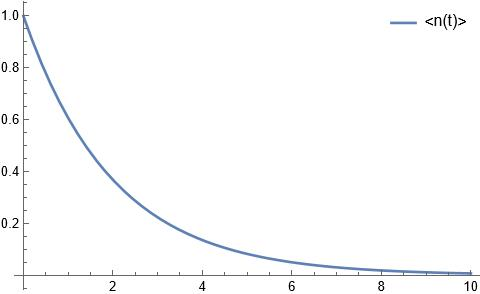
\includegraphics[width=0.6\linewidth]{NAnalitical.JPG}
		\caption{Average number of particles}
	\end{figure}
	
	The evolution of the average number of particles is shown in Fig.~\ref{fig:NAv}
	
		The same results are obtained for the average linear operators.
	
	We can also compare these results for the case when the higher order moments in Eq.~\eqref{eq:FinDinOfAv} are written out via Wick's theorem.
	
	\begin{figure}[h!]
		\begin{center}
			\begin{minipage}[h]{0.45\linewidth}
				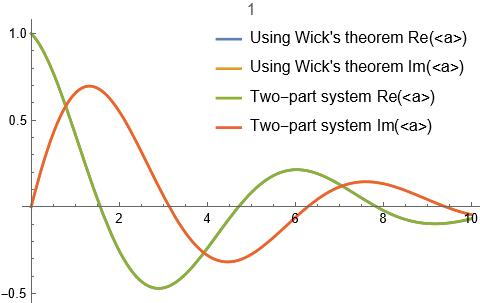
\includegraphics[width=1\linewidth]{Wickn0=1.JPG}
				\caption{Comparison with initial number of particles = 1}
				\label{fig:wick1}
			\end{minipage}
			\hfil
			\begin{minipage}[h]{0.45\linewidth}
				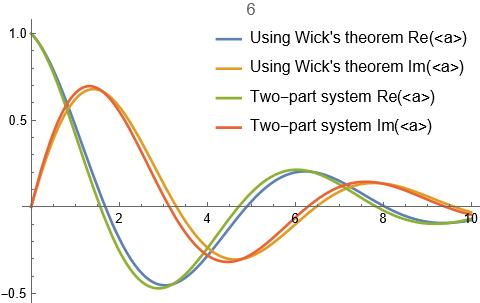
\includegraphics[width=1\linewidth]{Wickn0=6.JPG}
				\caption{Comparison with initial number of particles = 6}
				\label{fig:wick6}
			\end{minipage}
		\end{center}
	\end{figure}
	
	As can be seen in Fig.~\ref{fig:wick1}, for the number of particles equal to 1, both methods give the same result, however, as the number of particles increases, they begin to decay, so the analytical results were obtained for two partial approximation and it stops working Fig.~\ref{fig:wick6}.
	
	\section{Weak external field\label{sec:Efc}}
	
	In this section we consider the case when an external field is present in the system, i.e. $F \not= 0$. However, considering the general case is a difficult task due to the large number of summands in the oscillator, so we consider the case where the external field is small and the summands with $F^{1 + n}$, $n > 0$ can be neglected. 
	
	\begin{align}
		\label{eq:GenIntWithF}
		\mathcal{L}(t)\cdot &= -i\frac{\chi}{2}(({a^+}^2a^2\cdot) - (\cdot{a^+}^2a^2) + 2(e^{-\frac{\ga}{2}t} -1 ) [({a^+}a^2\cdot {a^+}) - (a\cdot{a^+}^2a) ] +2a_1^2b_2a_{21}({a^+}a^2\cdot) \nonumber\\
		&+ (2a_1^2b_2a_{22} - 2b_3a_3a_{42}^2)(a^2\cdot{a^+}) + 2b_1a_1 [a_{21}^2({a^+}^2a\cdot) + 2a_{21}a_{22}({a^+}a\cdot{a^+})] - 2a_3^2b_4a_{41}(\cdot{a^+}^2a) \\
		&+ (2b_1a_1a_{22}^2 - 2a_3^2b_4a_{42})(a\cdot{a^+}^2) - 2b_3a_3[a_{41}^2(\cdot{a^+}a^2) + 2 a_{41}a_{42}(a\cdot{a^+}a)) ]\nonumber,
	\end{align}
	where
	\begin{align*}
		a_1 &= e^{-\frac{\gamma  t}{4}+i \Delta  t}, \quad
		b_1 = \frac{F \left(4-4 e^{-\frac{\gamma  t}{4}+i \Delta  t}\right)}{\gamma -4 i \Delta }, \quad
		a_{21} = e^{\frac{1}{4} t (\gamma -4 i \Delta )}, \quad
		a_{22} = -2 e^{-i \Delta  t} \sinh \left(\frac{\gamma  t}{4}\right),\\
		b_2 &= \frac{F \left(4-4 e^{-\frac{1}{4} t (\gamma +4 i \Delta )}\right)}{\gamma +4 i \Delta }, \quad
		a_3 = e^{-\frac{1}{4} t (\gamma +4 i \Delta )}, \quad
		b_3 = \frac{F \left(4-4 e^{-\frac{1}{4} t (\gamma +4 i \Delta )}\right)}{\gamma +4 i \Delta }, \quad
		a_{41} = e^{\frac{1}{4} t (\gamma +4 i \Delta )},\\
		a_{42} &= -2 e^{i \Delta  t} \sinh \left(\frac{\gamma  t}{4}\right), \qquad
		b_4 = \frac{F \left(4-4 e^{-\frac{\gamma  t}{4}+i \Delta  t}\right)}{\gamma -4 i \Delta }.
	\end{align*}
	
	In this case, the action of the conjugate oscillator on an expression of type ${a^+}^na^m$ has the form
	
	\begin{align}
		\label{eq:ActOfGenOnExpr}
		\mathcal{L}^*(t){a^+}^na^m &= -i\frac{\chi}{2}(c_{00}{a^+}^na^m + c_{11}{a^+}^{n+1}a^{m+1} c_{01}{a^+}^na^{m + 1} + c_{12}{a^+}^{n + 1}a^{m + 2} \nonumber\\&+ c_{0-1}{a^+}^na^{m-1} + c_{-10}{a^+}^{n - 1}a^m + c_{10}{a^+}^{n+1}a^m + c_{21}{a^+}^{n+2}a^{m+1}),
	\end{align}
	where
	\begin{align*}
		c_{00} &= m (m-1)-n (n-1), \qquad
		c_{11} = 2 (m-n) e^{\frac{1}{2} (-\gamma ) t}, \\
		c_{01} &= 2 {a_1}^2 {a_{21}} {b_2} m-4 {a_3} {a_{41}} {b_3} n ({a_{41}}+{a_{42}}),\\
		c_{12} &= 2 {a_1}^2 {a_{21}} {b_2}+2 \left({a_1}^2 {a_{22}} {b_2}-{a_3} {a_{42}}^2 {b_3}\right)-2 {a_3} {a_{41}} {b_3} ({a_{41}}+2 {a_{42}}),\\
		c_{0-1} &= 2 {a_1} {a_{21}}^2 {b_1} m (m-1),\qquad
		c_{-10} =-2 {a_3} {a_{41}}^2 {b_3} n (n-1),\\
		c_{10} &= 4 {a_1} {a_{21}} {b_1} m ({a_{21}}+{a_{22}})-2 {a_3}^2 {a_{41}} {b_4} n,\\
		c_{21} &= 2 {a_1} {a_{21}} {b_1} ({a_{21}}+2 {a_{22}})+2 \left({a_1} {a_{22}}^2 {b_1}-{a_3}^2 {a_{42}} {b_4}\right)-2 {a_3}^2 {a_41} {b_4}.
	\end{align*}
	As we see, in this case such operator does not give an identical 0 when acting on the particle number operator.
	
	
	
	\begin{figure}[h!]
		\begin{center}
			\begin{minipage}[h]{0.45\linewidth}
				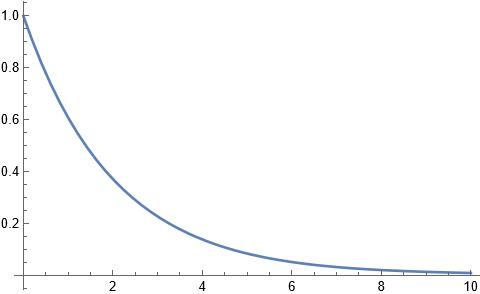
\includegraphics[width=1\linewidth]{NWeakForce.JPG}
				\caption{Average number of particles in the weak field}
				\label{fig:weakforcen}
			\end{minipage}
			\hfil
			\begin{minipage}[h]{0.45\linewidth}
				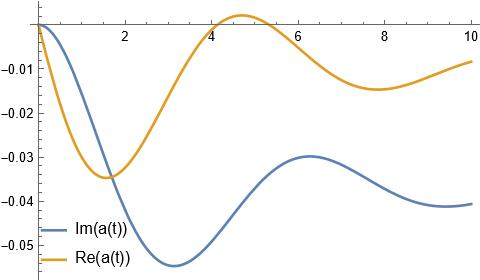
\includegraphics[width=1\linewidth]{aWeakForce.JPG}
				\caption{Mean of the linear operator in a weak field}
				\label{fig:weakforcea}
			\end{minipage}
			\hfil
			\begin{minipage}[h]{0.45\linewidth}
				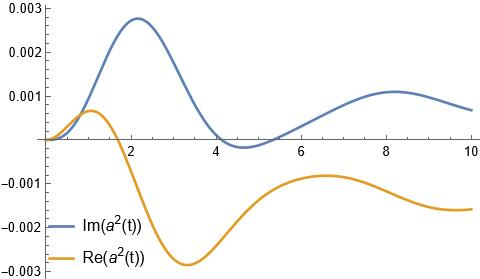
\includegraphics[width=1\linewidth]{a2WeakForce.JPG}
				\caption{Mean of the quadratic operator in a weak field}
				\label{fig:weakforceaa}
			\end{minipage}
		\end{center}
	\end{figure}
	
	We can also compare the difference between our method and the method using only Wick's theorem in  Eq.~\eqref{eq:FinDinOfAv}. This can be done by calculating our equation with $F = 0$. Once we have done this, we can compare the results. The results are presented in Fig. \ref{fig:compn} \ref{fig:compa} \ref{fig:compa2}
	
	
	\begin{figure}[h!]
		\begin{center}
			\begin{minipage}[h!]{0.45\linewidth}
				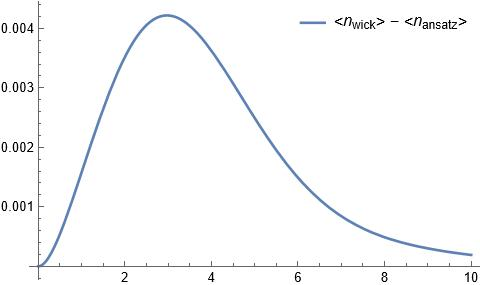
\includegraphics[width=1\linewidth]{Comparen.JPG}
				\caption{Comparison of results for average particle number}
				\label{fig:compn}
			\end{minipage}
			\hfil
			\begin{minipage}[h!]{0.45\linewidth}
				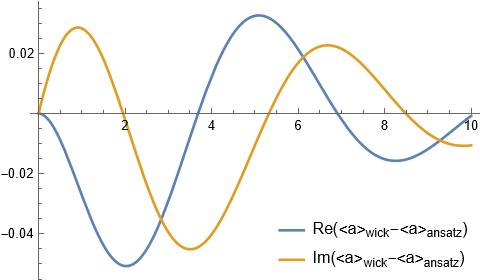
\includegraphics[width=1\linewidth]{Comparea.JPG}
				\caption{Comparison of results for Mean of the linear operator}
				\label{fig:compa}
			\end{minipage}
			\hfil
			\begin{minipage}[h!]{0.45\linewidth}
				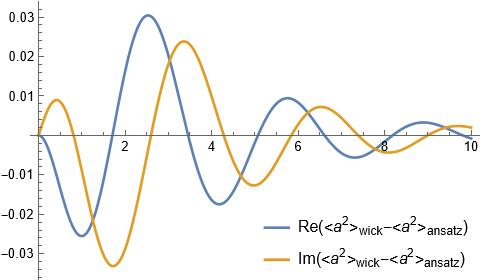
\includegraphics[width=1\linewidth]{Comparea2.JPG}
				\caption{Comparison of results for Mean of the quadratic operator}
				\label{fig:compa2}
			\end{minipage}
		\end{center}
	\end{figure}
	
	As can be seen, the results are of order $\la$, but for the quadratic operator the averages themselves are of the same order.
	
	
	\section{Conclusions}
	In this work, we have focused on obtaining the Gaussian approximation for the one-mode Kerr model in the external classical field with dissipation. But let us remark that the proposed technique is general and can be applied to multi-mode dissipative models, whose free dynamics preserves the Gaussian states. The specific choice of the model allows us to verify it in the regime, when it is exactly solvable with non-Gaussian solutions. So it can be used as a benchmark of our approach in such an ''uncomfortable'' case for it. And, at the same time, our approach allows us to obtain the dynamics for this model in the case, when it is not exactly solvable. This demonstrates the usefulness of our technique.
	
	As an obvious direction for the future study we should mention the application of our approach to other specific models, especially  multimode ones. Most of our general calculations are already done in multimode case. And the specific calculations for the discussed model do not seem to complicate much in the multimode case for any reasonable finite number of modes. 
	
	The other direction for the future study is to approximate the solution by the finite linear combinations of Gaussian states and applying our equations to each term in the combination separately. In case of non-convex linear combinations, it may allow one to take some non-Gaussian quantum effects into account.
 % It can be considered as analog for adapted projector technique (), but with non-linear ansatzes.
	
	
	
 \bibliographystyle{unsrt}
 \bibliography{ref}
%	
	%	\begin{thebibliography}{99}
	
	%		\bibitem{KerrIntr} Lorenc D., Alpichshev Z. Dispersive effects in ultrafast nonlinear phenomena: The case of optical Kerr effect //Physical Review Research. – 2024. – V. 6. – N. 1. – Pg. 013042.
	
	%		\bibitem{GaussState} Menu R., Roscilde T. Gaussian-state Ansatz for the non-equilibrium dynamics of quantum spin lattices //SciPost Physics. – 2023. – V. 14. – N. 6. – Pg. 151.
	
	%		\bibitem{Kholevo} A.S. Kholevo Quantum systems, channels, information. M.: MCNMO, 2010.
	
	%		\bibitem{MaslovN} Liu, Junqiu, et al. "High-yield, wafer-scale fabrication of ultralow-loss, dispersion-engineered silicon nitride photonic circuits." Nature communications 12.1 (2021): 2236.
	
	%		\bibitem{MaslovSolve} S.P. Nikitin, A.V. Masalov. Quantum state evolution of the fundamental mode in the process of second-harmonic generation. Quantum Optics 3, № 2, 105-113 (1991).
	
	%		\bibitem{Dis} Teretenkov A.E. (2018). Exactly solvable problems	irreversible quantum evolution
	
	%		\bibitem{NosalTeretenkov} Nosal Iu.A., Teretenkov A.E.  "Higher order moments dynamics for some multimode quantum master equations." Lobachevskii Journal of Mathematics 43.7 (2022): 1726-1739.
	
	%	\end{thebibliography}
	\newpage
	
	
	\section{Appendix\label{App}}
	
	
	
	% \begin{equation*}
	% 	I = \begin{pmatrix}
	% 		I_N & 0 \\
	% 		0 & I_N
	% 	\end{pmatrix}.
	% \end{equation*}
	
	% Also such notations allow to write the following expressions compactly
	
	% \begin{equation*}
	% 	\operatorname{tr} \mathfrak{a}^T f g^T  \mathfrak{a} \rho =   f^T \operatorname{tr}(\mathfrak{a}  \mathfrak{a}^T \rho) g = f^T D g = \Tr D g  f^T  = \Tr f g^T D^T
	% \end{equation*}
	% hence 
	% \begin{equation}
	% 	\label{eq:CompFormOfAv}
	% 	\operatorname{tr} \mathfrak{a}^TA \mathfrak{a} \rho  = \Tr AD^T
	% \end{equation}
	
%	The characteristic function of such ansatz has the form
%	
%	\begin{equation}
%		\chi(\textbf{z}) = \Tr(\rho_{anz} e^{\textbf{z}^T\mathfrak{a}}) =  e^{\frac{1}{2}(i\textbf{z}^T)C(i\textbf{z}) + i\textbf{z}^Tm}
%	\end{equation}
	
	Let us write out some of the beneficial properties of the Gaussian ansatz.
	
	\begin{theorem}
		\label{th:KvFor}
		\begin{align*}
			\label{eq:KvFor}
			e^{\dfrac{1}{2}\mf{a}^TK\mf{a} + g^T\mf{a}}(\dfrac{1}{2}\mf{a}^TM\mf{a} + f^T\mf{a})e^{-(\dfrac{1}{2}\mf{a}^TK\mf{a} + g^T\mf{a})} &= \dfrac{1}{2}\mf{a}^Te^{-KJ}Me^{JK}\mf{a} + \left(e^{-kJ}M\dfrac{e^{JK}-I}{JK}Jg + e^{-KJ}f\right)^T\mf{a} + \nonumber\\
			&+ \left(\dfrac{1}{2}g^TJ\dfrac{e^{-KJ}-I}{KJ}M + f^T\right)\dfrac{e^{JK} - I}{JK}Jg&
		\end{align*}
	\end{theorem}
	The proof can be found in \cite{Dis}. 
	
	This feature allows us to carry the density matrix through the quadratic form of the creation/annihilation operators.
	
	However, the main feature that is the reason we use the Gaussian ansatz is Wick's theorem.
	
	\begin{theorem}
		\label{th:IW0}
		For a Gaussian ansatz with zero mean and with the matrix of second moments $D$ it follows that 
		\begin{equation*}
			\braket{\mf{a}_I} = \sum\limits_{I = I_1 \sqcup I_2}\mu_{I_1}D_{I_2}.
		\end{equation*}
	\end{theorem}
	The proof of this theorem and more details can be found in \cite{NosalTeretenkov}
	
	
	
	
	%	\section{\label{sec:QuadraticForm} Quadratic form}
	
	\begin{theorem}
		\label{th:HeiGenerator}
		The generator $\mathcal{L}(t)\rho = -i[H_{\lambda},\rho] + \dfrac{\ga}{2}(a\rho a^+ - \dfrac12\{a^+a,\rho\}),$ in the Heisenberg representation has the form 
		\begin{equation*}
			\mathcal{L}^*\rho = i[H_{\la},\rho]  + \dfrac{\ga}{2}(a^+\rho a - \dfrac{1}{2}\{a^+a,\rho\}\}).
		\end{equation*}
	\end{theorem}
	
	\begin{demo}
		The operator $\mathcal{L}$ can be represented as $\mathcal{L} = \sum X_i\cdot Y_i$, then 
		
		\begin{equation*}
			\Tr(A\mathcal{L}B) = \sum\Tr(AX_i(B)Y_i)
		\end{equation*}
		
		Since the trace is invariant with respect to cyclic permutations, then 	
		
		\begin{equation*}
			\sum\Tr(AX_i(B) Y_i) = \sum\Tr(B Y_i(A)X_i) = \sum\Tr(B(Y_i\cdot X_i)(A)),
		\end{equation*}
		hence the operator $\mathcal{L}^*$ is represented in the form $\mathcal{L}^* = \sum Y_i \cdot X_i$
		
		
		The operator $\mathcal{L}$ can be rewritten as
		
		\begin{equation*}
			\mathcal{L}(B) = -i(HB\mathcal{I} - \mathcal{I}B H) + \dfrac{\ga}{2}(aB a^+ - \dfrac{1}{2}[a^+aB\mathcal{I} + \mathcal{I}B a^+a]),
		\end{equation*}
		hence
		
		\begin{equation*}
			Y(A)X = -iAH + iHA + \dfrac{\ga}{2}(a^+Aa - \dfrac{1}{2}[Aa^+a + a^+aA]),	
		\end{equation*}
		Thus we get the desired result.
	\end{demo}
	
	\begin{theorem}
		\label{th:DerOfGaus}
		The derivative of the Gaussian exponent can be expressed as a quadratic form
		
		\begin{equation*}
			\frac{d}{dt}\rho_{anz} = (\frac{1}{2}\mf{a}^TM\mf{a} + \mf{a}^TG + c)\rho_{anz},
		\end{equation*}
		where
		\begin{align*}
			M &= \frac{I}{C - \frac{J}{2}}\left(\frac{d}{dt}C\right)\frac{I}{C + \frac{J}{2}},\\
			G &= \left(  I + \frac{2I}{2J^{-1}C - I}  \right)\frac{d}{dt}\left(\frac{I}{C + \frac{J}{2}}m\right),\\
			c &=-m^T\frac{I}{2J^{-1}C -  I}\frac{d}{dt}\left(\frac{I}{C + \frac{J}{2}}m\right) + \frac{1}{2}\frac{d}{dt}m^T\left( \frac{I}{2J^{-1}C - I} - \frac{I}{2J^{-1}C + I} - KJ \right)J^{-1}m + \frac{d}{dt}c_t,
		\end{align*}
		where $g = -Km$, in which $m = (\braket{a} , \braket{a^+})^T$ and $C$ --- covariance matrix.
	\end{theorem}
	\begin{demo}
		The formula for the derivative of Gaussian ansatz can be found in \cite{Dis}
		\begin{equation}
		%	\label{eq:DerWithLin}
			\frac{d}{dt}\rho_{anz} = (\mf{a}^TM\mf{a} + \mf{a}^TG + c)\rho_{anz},
		\end{equation}
		where
		\begin{align*}
			M &= \frac{1}{2}\frac{I}{C - \frac{J}{2}}\left(\frac{d}{dt}C\right)\frac{I}{C + \frac{J}{2}},\\
			G &= e^{-KJ}\frac{d}{dt}\left(\frac{e^{KJ} - I}{KJ}g\right),\\
			c &= \frac{1}{2}g^TJ\frac{e^{-KJ} - I}{KJ}\frac{d}{dt}\left( \frac{e^{KJ} - I}{KJ}g  \right) + \frac{d}{dt}\left(  \frac{1}{2}g^T\frac{J}{KJ}(\text{sh}(KJ) - KJ)\frac{1}{KJ}g  +c_t \right).
		\end{align*}
		
		
		Using the formula $\text{arcoth}(x) = \frac{1}{2}\ln\left(\frac{x + 1}{x - 1}\right)$, we can explicitly write $e^{KJ}$.
		
		\begin{equation*}
			e^{KJ} = \frac{2J^{-1}C - I}{2J^{-1}C + I} = I - \frac{2I}{2J^{-1}C + I},
		\end{equation*}
		then
		\begin{align*}
			e^{-KJ}\frac{d}{dt}e^{KJ}J^{-1} =& -2\frac{2J^{-1}C + I}{2J^{-1}C - I}\frac{d}{dt}(2J^{-1}C + I)^{-1}J^{-1} = \\
			&4 \frac{2J^{-1}C + I}{2J^{-1}C - I} \frac{I}{2J^{-1}C + I}J^{-1}\left(\frac{d}{dt}C\right)\frac{I}{2J^{-1}C + I}J^{-1} = \\
			& 4 \frac{I}{2J^{-1}C - I}J^{-1}\left(\frac{d}{dt}C\right)\frac{I}{2J^{-1}C + I}J^{-1} = \frac{I}{C - \frac{J}{2}}\left(\frac{d}{dt}C\right)\frac{I}{C + \frac{J}{2}}
		\end{align*}
		
		In a similar way, we can simplify the vector $G$
		
		\begin{align*}
			G &= e^{-KJ}\frac{d}{dt}\left(\frac{e^{KJ} - I}{KJ}g\right) = \left(  I + \frac{2I}{2J^{-1}C - I}  \right)\frac{d}{dt}\left( \frac{
				\frac{2J^{-1}C - I}{2J^{-1}C + I} - I}{KJ}   g  \right) =\nonumber\\
			& = \left(  I + \frac{2I}{2J^{-1}C - I}  \right)\frac{d}{dt}\left( \frac{2I}{2J^{-1}C + I} J^{-1}m  \right) = \left(  I + \frac{2I}{2J^{-1}C - I}  \right)\frac{d}{dt}\left(\frac{I}{C + \frac{J}{2}}m\right).
		\end{align*}
		
		\begin{align*}
			&\frac{1}{2}g^TJ\frac{e^{-KJ} - I}{KJ}\frac{d}{dt}\left( \frac{e^{KJ} - I}{KJ}g  \right) = \frac{1}{2}g^TJ\frac{e^{-KJ} - I}{KJ}\frac{d}{dt}\left(\frac{I}{C + \frac{J}{2}}m\right) =\nonumber\\
			&=-\frac{1}{2}m^TKJ(KJ)^{-1}\left(I + 2\frac{I}{2J^{-1}C - I} - I\right)\frac{d}{dt}\left(\frac{I}{C + \frac{J}{2}}m\right) = -m^T\frac{I}{2J^{-1}C -  I}\frac{d}{dt}\left(\frac{I}{C + \frac{J}{2}}m\right)
		\end{align*}
		
		\begin{align*}
			\text{sh}(KJ) = \frac{I - \frac{2I}{2J^{-1}C + I} - I + \frac{2I}{2J^{-1}C - I}}{2} = \frac{I}{2J^{-1}C - I} - \frac{I}{2J^{-1}C + I}
		\end{align*}
		
		\begin{align*}
			&\frac{d}{dt}\left(  \frac{1}{2}g^TJ\frac{I}{KJ}(\text{sh}(KJ) - KJ)\frac{1}{KJ}g\right) = \frac{1}{2}\frac{d}{dt}m^T(\text{sh}(KJ) - KJ)J^{-1}m = \nonumber\\
			&\frac{1}{2}\frac{d}{dt}m^T\left( \frac{I}{2J^{-1}C - I} - \frac{I}{2J^{-1}C + I} - 2\text{arcoth}(-2J^{-1}C) \right)J^{-1}m
		\end{align*}
		
		\begin{align*}
			c = -m^T\frac{I}{2J^{-1}C -  I}\frac{d}{dt}\left(\frac{I}{C + \frac{J}{2}}m\right) + \frac{1}{2}\frac{d}{dt}m^T\left( \frac{I}{2J^{-1}C - I} - \frac{I}{2J^{-1}C + I} - KJ \right)J^{-1}m + \frac{d}{dt}c_t
		\end{align*}
		where
		
		\begin{equation}
			\label{eq:c}
			e^{c_t} = \left(\Tr e^{\frac{1}{2} \mathfrak{a}^TK\mathfrak{a} + g^T\mf{a}}\right)^{-1} = \sqrt{\left|\text{det}(e^{KJ} - I)\right|}e^{\frac{1}{2}g^TK^{-1}g}.
		\end{equation}
	\end{demo}
	
	\begin{theorem}
		\begin{equation*}
%			\label{eq:RhoSq}
			\rho_{0,C}^2 = \frac{1}{\sqrt{|\det(2 C)|}} \rho_{0,C'}.
		\end{equation*}
		where 
		\begin{equation*}
			C' = - \frac{J}{4}\left(\frac{1}{2 J C} + 2 J C\right).
		\end{equation*}
	\end{theorem}
	\begin{demo}
		\begin{equation*}
			\rho_{0,C}^2 = \frac{Z'}{Z^2}\rho_{0,C'},
		\end{equation*}
		where 
		
		\begin{equation*}
			Z = \operatorname{tr} e^{\frac12 \mathfrak{a}^T K  \mathfrak{a}}  = \frac{1}{\sqrt{|\det(e^{KJ} - I)|}},
		\end{equation*}
		
		\begin{equation*}
			Z' = \operatorname{tr} e^{\frac12 \mathfrak{a}^T 2K  \mathfrak{a}}  = \frac{1}{\sqrt{|\det(e^{2KJ} - I)|}}.
		\end{equation*}
		
		Then 
		
		\begin{equation*}
			\frac{\operatorname{tr} e^{\frac12 \mathfrak{a}^T 2K  \mathfrak{a}}  }{(\operatorname{tr} e^{\frac12 \mathfrak{a}^T K  \mathfrak{a}})^2} = \sqrt{\left|\det\left(\frac{(e^{KJ} - I)^2}{e^{2 KJ} - I}\right)\right|}
		\end{equation*}
		
		\begin{equation*}
			\frac{(e^{KJ} - I)^2}{e^{2 KJ} - I} = \frac{e^{KJ} - I}{e^{KJ} + I} = \frac{1}{\coth \frac{KJ}{2}} = \frac{1}{-2J^{-1} C}
		\end{equation*}
		
		\begin{equation*}
			\frac{\operatorname{tr} e^{\frac12 \mathfrak{a}^T 2K  \mathfrak{a}}  }{(\operatorname{tr} e^{\frac12 \mathfrak{a}^T K  \mathfrak{a}})^2} = \sqrt{\left|\det\left(\frac{1}{-2J^{-1} C}\right)\right|} = \frac{1}{\sqrt{|\det(2 C)|}}
		\end{equation*}
	\end{demo}
\end{document} 